\documentclass[12pt]{article}

%%% Packages %%%

\usepackage{amsmath}
\usepackage{amssymb}
\usepackage{amsthm}

\usepackage[dvipsnames]{xcolor}

%%% Formatting/Configs %%%

\setlength{\parindent}{0pt}
\setlength{\parskip}{6pt}

%%% Macros %%%

\newcommand{\N}{\mathbb{N}}
\newcommand{\Z}{\mathbb{Z}}
\newcommand{\Q}{\mathbb{Q}}
\newcommand{\R}{\mathbb{R}}
\newcommand{\C}{\mathbb{C}}

\newcommand{\X}{\mathfrak{X}}
\newcommand{\Cinf}{C^\infty}
\newcommand{\T}{\mathrm{T}}
\newcommand{\TT}{\mathfrak{T}}

\newcommand{\ccdot}[1][]{\,\cdot\,}

\let\d\relax
\DeclareMathOperator{\d}{d}
\newcommand{\di}[1][]{\operatorname{d}_{#1}\def\temp{#1}\!}
\DeclareMathOperator{\id}{id}


%%% Elias' crap %%%

\newcommand{\todo}[1]{\textcolor{NavyBlue}{[todo: #1]}}
\newcommand{\beware}[1]{\textcolor{Red}{[beware: #1]}}
\newcommand{\question}[1]{\textcolor{Green}{[question: #1]}}

%%% Environments %%%

\theoremstyle{definition}
\newtheorem*{definition}{Definition}
\newtheorem*{example}{Example}
\newtheorem*{notation}{Notation}

\theoremstyle{plain}
\newtheorem*{thm}{Theorem}
\newtheorem*{prop}{Proposition}
\newtheorem*{lemma}{Lemma}
\newtheorem*{cor}{Corrolary}

\theoremstyle{remark}
\newtheorem*{remark}{Remark}


\begin{document}

\begin{titlepage}
   \begin{center}
       \vspace*{4cm}

       {\LARGE
       \bf
       A Short Introduction into Singular Foliations from the Perspective of Partitionifolds

       \vspace{1cm}

       {\large
       \textbf{Elias Garcia-Naze \& Max Sundblad}

       \vspace{0.5cm}

       July 2025
   \end{center}
\end{titlepage}

\tableofcontents

\newpage

\section{Introduction}
    Singular foliations are a generalization of regular foliations in which leaves are allowed to have different dimensions. Whilst regular foliations have sparked great interest and research for a long time, singular foliations have not been as comprehensively studied until very recently. This might have to do with the difficulty of finding a good definition for them. This is precisely the mission which was undertaken by a few mathematicians in the 60s and 70s. After the research into the topic lost its impetus and lay dormant until 2000s when singular foliations saw a sort of revival coming from non-commutative geometry.

    In this report we will study singular foliations from the lens of so called partitionifolds. We will first look at their general case and then also with a sort of smooth condition imposed on them.

\section{Notations and definitions}
    In this section we recall some of the basic definitions of differential geometry and introduce the notation we're gonna use in the rest of the report, especially about tangent spaces vector fields.

    Throughout this report the letter $M$ will be reserved for a manifold of dimension $d$.

	Now we recall one of the definitions of a tangent vector.

	\begin{definition}
		Let $m \in M$.
		We call \textbf{tangent space of $M$ at the point $m$} (written $\T_m{M}$) the set of ``\emph{directional derivatives}'', or rather ``\emph{path derivatives}'' (the direction is described by a smooth path in $M$).
        
		This means that any \textbf{tangent vector} $v \in \T_m{M}$ is a function $v: \Cinf(M) \to \R$ defined by
		$$
			\forall f \in \Cinf(M), \quad v(f) = \frac{\d}{\di{t}} f(\gamma(t)) \Big|_{t=0}
		$$
		for a path $\gamma \in \Cinf(\R, M)$ such that $\gamma(0) = m$.
	\end{definition}

	\begin{notation}
		Let $\gamma \in \Cinf(J, M)$ (where $J \subset \R$ is an open subset, often taken to be an interval), and $t_0 \in J$.
		As a shorthand for the path derivative along $\gamma$ at time $t_0$ of a function $f \in \Cinf(M)$ we write 
		$$
			\frac{\partial f}{\partial \gamma}(t_0) := \frac{\d}{\di{t}} f(\gamma(t)) \Big|_{t=t_0}
		$$

		Meaning that for any $m \in M$ a tangent vector $v \in \T_m{M}$ is of the form
		$$
			v = \frac{\partial \bullet}{\partial \gamma}(0)
		$$
		for a path $\gamma \in \Cinf(\R, M)$ such that $\gamma(0) = m$.
	\end{notation}

	\todo{local form, standardization}

	Let's define the tangent bundle quickly

	\todo{tangent bundle}
    
	\todo{how do we organize this?}

	\subsection{Tangent space}
        

	\subsection{Vector field}

	\subsection{Tangent map and diffeomorphisms}

	\subsection{Other (things used everywhere)}
        

		\todo{do we keep this, what do we put here?}

		\begin{itemize}
			\item M
			\item J
		\end{itemize}


\section{A first approach: Partitionifolds}

	Here we introduce the notion of partitionifold, give some examples, non-examples and properties. We also show {\color{Red}one of the principal shortcomings} of this first definition partitionifold, that'll motivate the introduction of smooth partitionifolds in the next section.

	\begin{definition}
		A \textbf{partitionifold} of $M$ is a partition of $M$ into \emph{connected immersed submanifolds} called \textbf{leaves} of the partitionifold.

		We write the partitionifold as $(M, L_\bullet)$, or simply $L_\bullet$, where $L_\bullet$ is the partition map
		$$
			L_\bullet : M \to \mathcal{P}(M), \quad m \mapsto L_m
		$$
		($L_m$ is the leaf containing the point $m$).

		\todo{If not specified otherwise ``$L_\bullet$'' will be considered to be a partitionifold of $M$.}
	\end{definition}

	This definition is built from the fact that a regular foliation indeed gives a partition of the manifold into immersed submanifolds \todo{talk about rank}. However we can already see some examples of partitionifold that don't come from regular foliations, even though every leaf has the same dimension \todo{point out the singularities}.

	\begin{example}[``T'' partitionifold]
		We can consider the partitionifold of $\R^2$ given by
		$$
		\begin{cases}
			L_{(x,y)} = \R \times \{y\}            &\text{ if } y \geq 0 \\
			L_{(x,y)} = \{x\} \times (-\infty, 0)  &\text{ if } y < 0
		\end{cases}
		$$

		\begin{figure}[H]
		    \centering
		    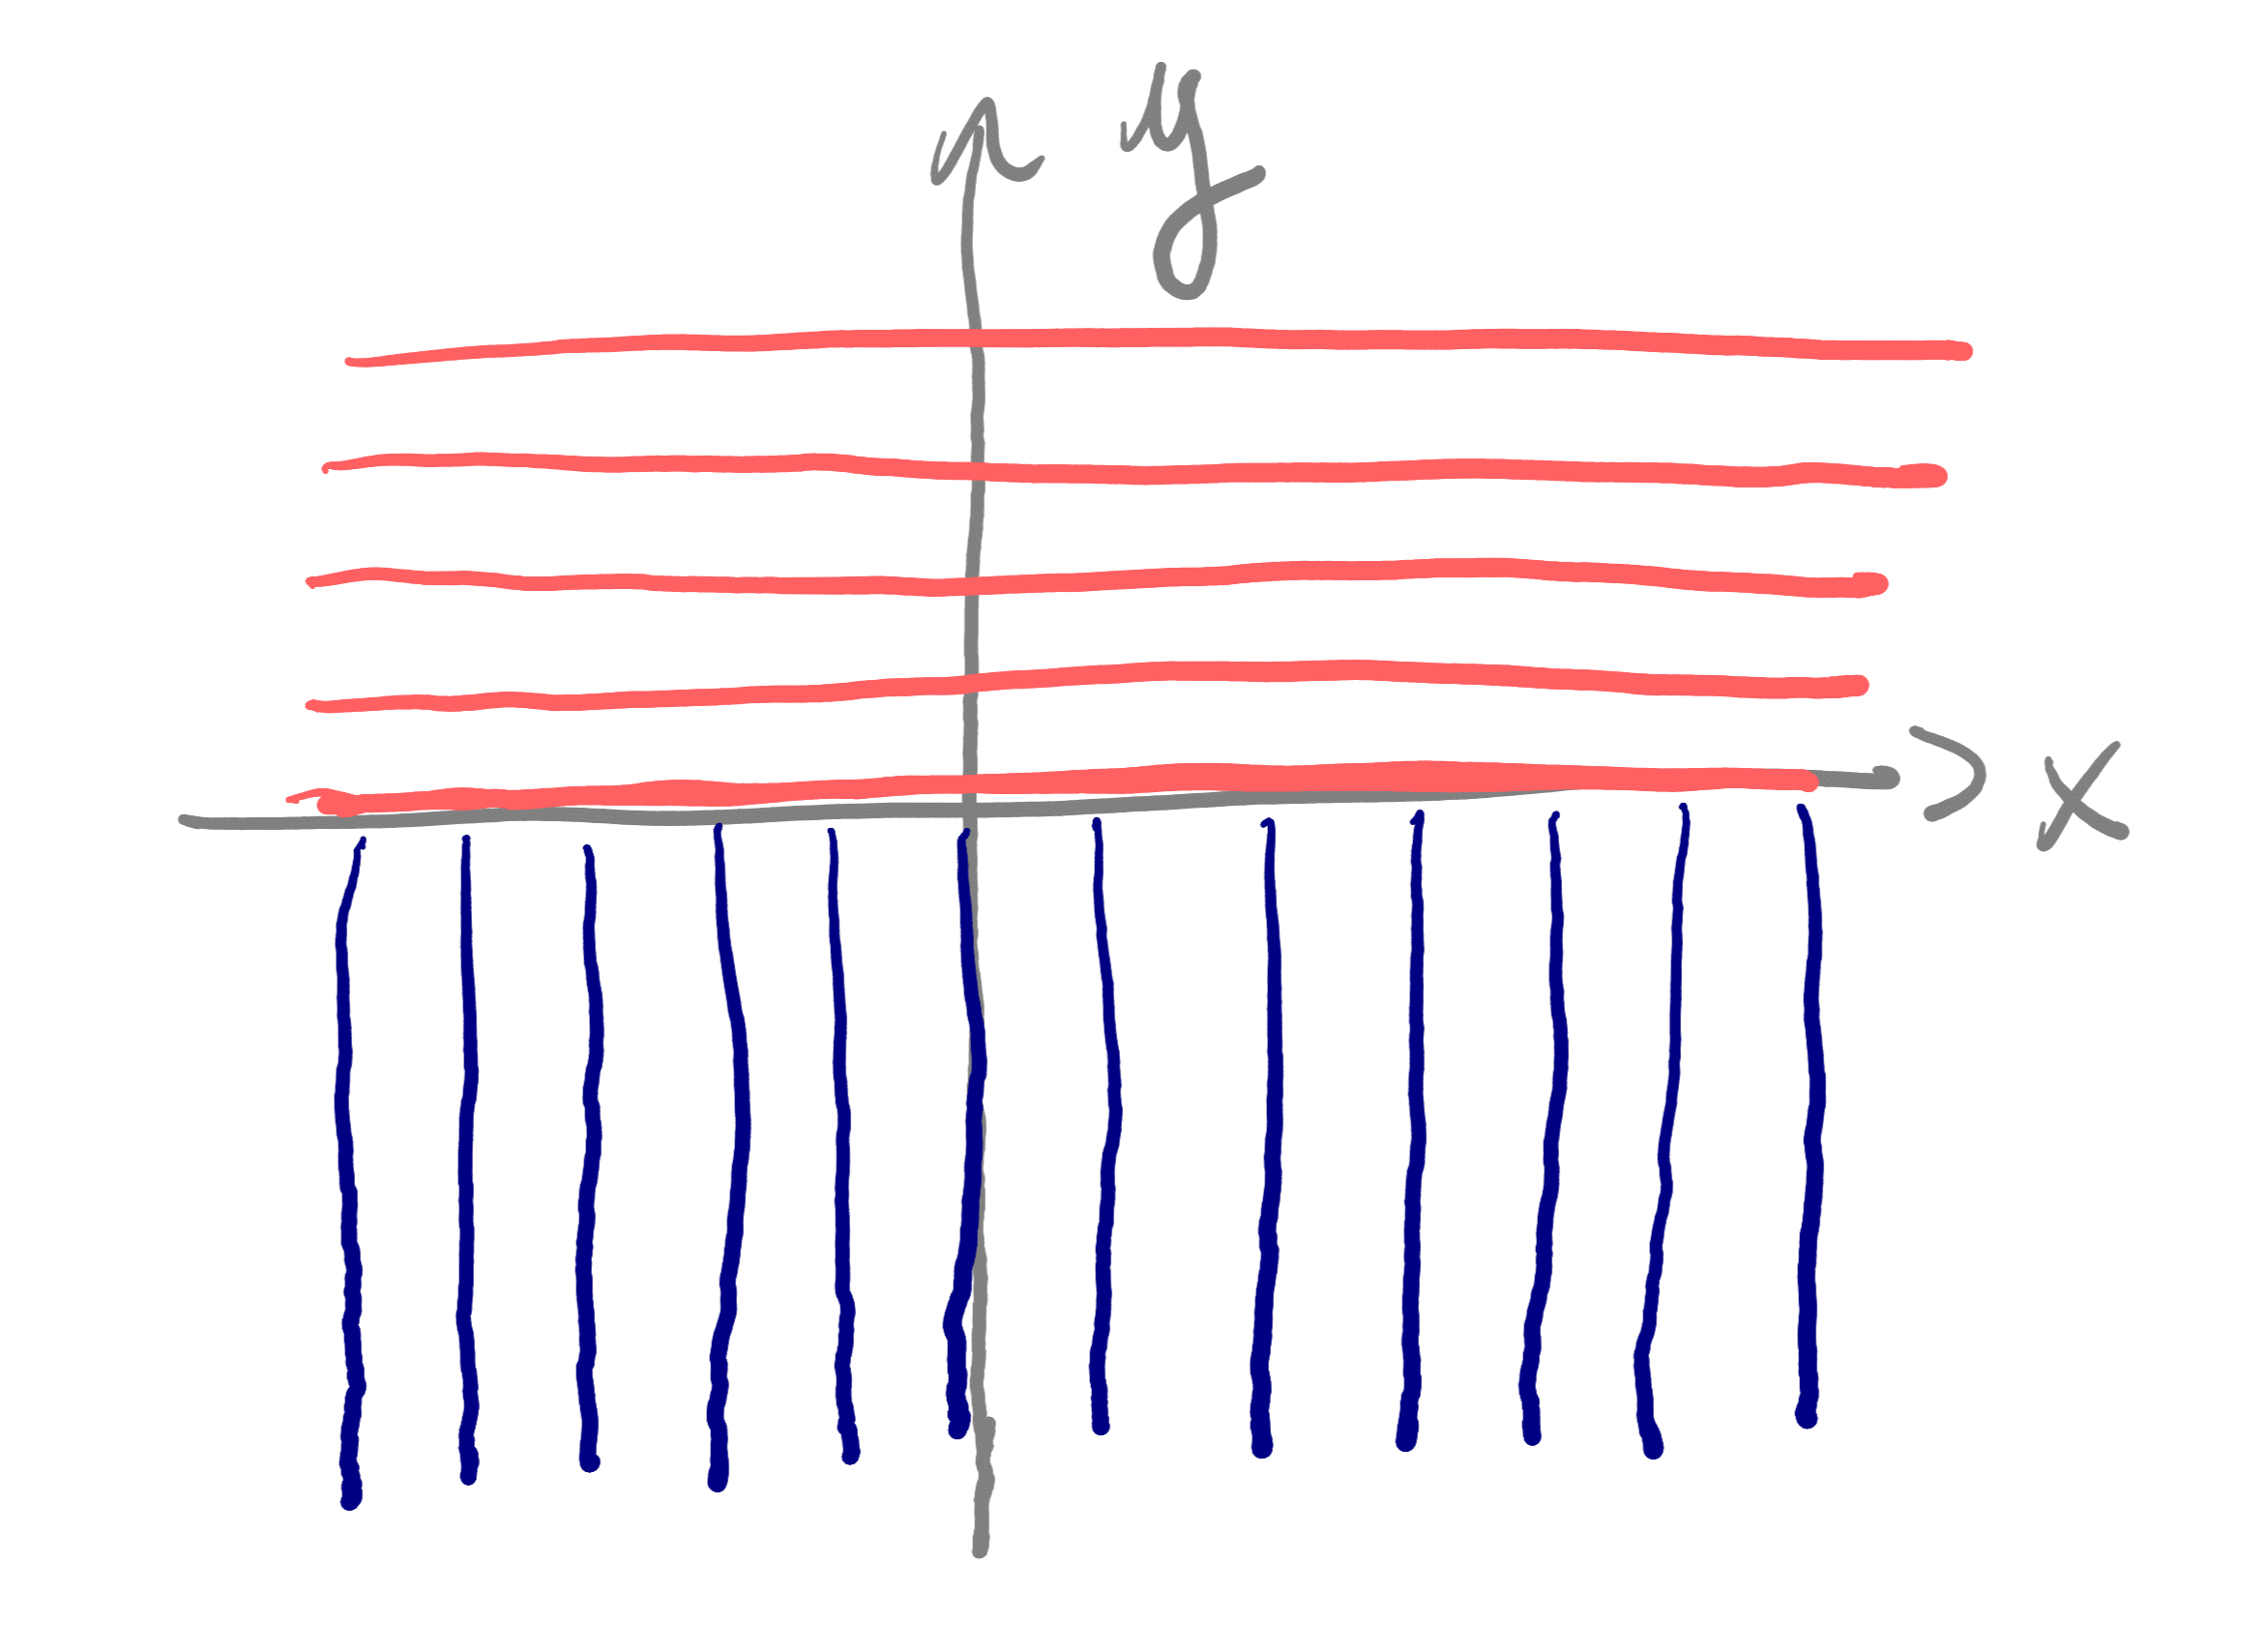
\includegraphics[width=0.8\linewidth]{T-foliation.png}
		    \caption{"T"-partitionifold}
		    \label{fig:enter-label}
		\end{figure}
	\end{example}

	\begin{example}[Circle covering of $\R^3$]
		It is possible to fill $\R^3$ with disjoint circles. 
	\end{example}

    \begin{example}[Isolated lasagna]
        The following is a partitionifold of $\R^3$:
%
        \begin{align*}
            \begin{cases}
                L_{(0, 0, 0)} = \R^2 \times \{0\} \\
                L_{(0, y, z)} = \R \times \{y\} \times\{z\} &\text{if $z \neq 0$} 
            \end{cases}
        \end{align*}
    \end{example}

	A really inconvenient thing about this definition is that a path $\gamma : J \to \R$ that is tangent to the leaf $L_{\gamma(t)}$ at any time $t \in J$ isn't guaranteed to be contained in a single leaf.

	\begin{example}
		In the ``T'' partitionifold, we can consider the path
		$$
			\gamma: t \in \R \mapsto
			\begin{cases}
				(e^{-1/t^2}, 0)  &\text{ if } t < 0 \\
				(0, 0)           &\text{ if } t = 0 \\
				(0, e^{-1/t^2})  &\text{ if } t > 0 \\
			\end{cases}
		$$

		We have
		$$
			\gamma'(t) =
			\begin{cases}
				(\frac{1}{t^3} e^{-1/t^2}, 0)  &\text{ if } t < 0 \\
				(0, 0)                         &\text{ if } t = 0 \\
				(0, \frac{1}{t^3} e^{-1/t^2})  &\text{ if } t > 0 \\
			\end{cases}
		$$
		
		The derivative of $\gamma$ at $t=0$ is in fact $0$ as specified since:
		$$
			\lim_{t \to 0^-} \frac{1}{t} e^{-1/t^2} = 0 = \lim_{t \to 0^+} -\frac{1}{t} e^{-1/t^2}
		$$

		We can see that for any $t \in \R$ we indeed have $\gamma'(t) \in \T_\gamma(t) L_{\gamma(t)}$.
        
		For $t \leq 0$ we have $\gamma(t) \in \R \times \{0\}$ and
		$$
			\gamma'(t) \in \R \times \{0\} = \T_{\gamma(t)}\big( \R \times \{0\} \big)
		$$
		For $t > 0$ we have $\gamma(t) \in \{0\} \times (-\infty, 0)$ and
		$$
			\gamma'(t) \in \{0\} \times \R = \T_{\gamma(t)}\big( \{0\} \times (-\infty, 0) \big)
		$$
	\end{example}

	In this example we see that we use the point $(0,0)$, which is in the adherence of the two leaves $\R \times \{0\}$ and $\{0\} \times (-\infty, 0)$, to pivot from one leaf to the other by using a path whose derivative vanishes at time $t=0$ ($\gamma(t) = (0,0)$)

	But you can even find a partitionifold which admits a smooth curve $\gamma: \R \to M$ with a derivative vanishing for some $t$ can then switch between any leaves that have the point $m = \gamma(t)$ in their adherence.

	\begin{example}[Spaghetti hooks]
		We consider the partitionifold of $\R^2$ given by
		$$
		\begin{cases}
			L_{(x,y)} = \R \times \{y\}            &\text{ if } y \leq 0 \quad \text{(the spaghetti)} \\
			\text{As in figure \ref{spaghetti-hooks}}
		\end{cases}
		$$
	\end{example}

    \begin{figure}[H]
        \centering
        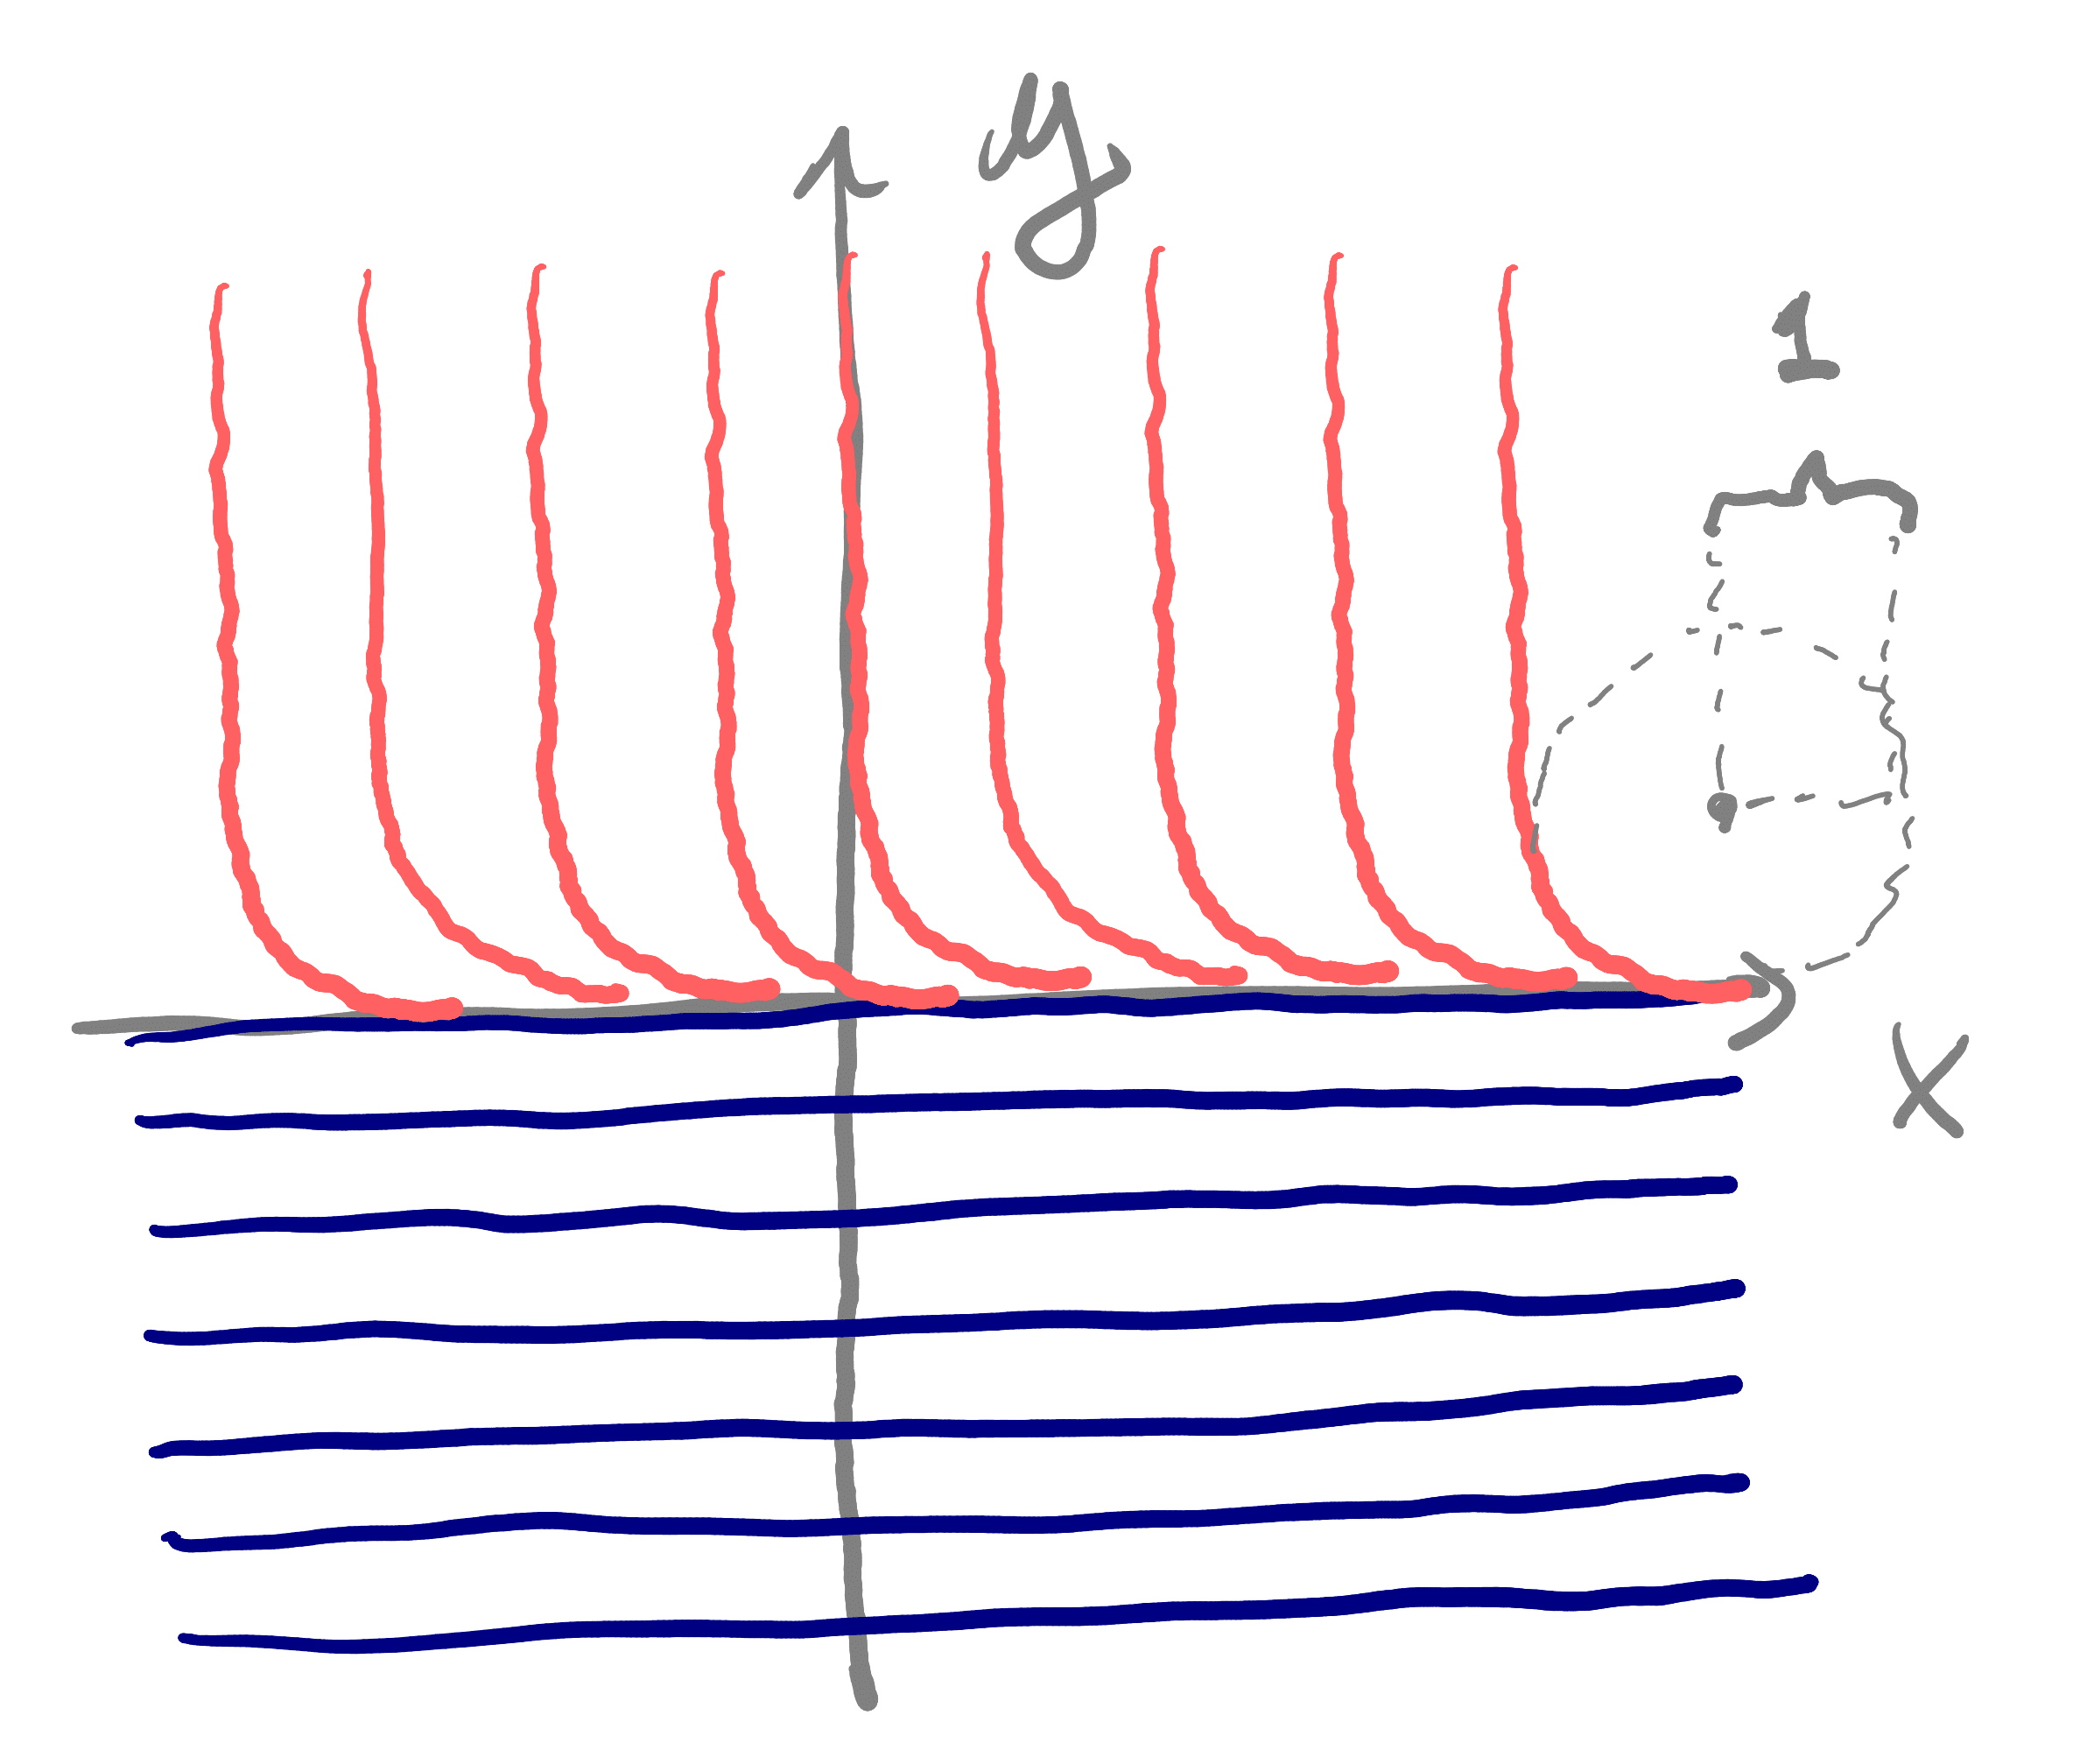
\includegraphics[width=0.7\linewidth]{spaghetti-hook.png}
        \caption{Spaghetti hook foliation}
        \label{spaghetti-hooks}
    \end{figure}

    \begin{definition}
        A vector field $X$ is said to be \textbf{tangent to $L_\bullet$} if for each $m \in M$ we have that $X(m) \in T_m L_m$. We let $\mathfrak{T}(L_\bullet)$ be the set of all such vector fields on $M$.
    \end{definition}

    \begin{prop}[Not leaving leaves]
	   If there is a vector field $X \in \mathfrak{T}(L_\bullet)$ then all integral curves of $X$ lie in one and only one leaf of $L_\bullet$.
    \end{prop}

    \begin{proof}
        Let $X$ be a given vector field in $\in \mathfrak{T}(L_\bullet)$, that is:
        %
        \begin{align*}
            X(m) \in T_m L_m
        \end{align*}

        for all $m \in M$.

        Let $\gamma : I \to M$ be an integral curve of $X$:
        %
        \begin{align*}
            \frac{d \gamma}{dt}(t) = X(\gamma(t))
        \end{align*}

        which starts at $m_0 \in M$.

        Since $X|_{L_{m_0}}$ is in fact a vector field of $L_{m_0}$ we can find also an integral curve $\lambda$ of $X|_{L_{m_0}}$ starting at $m_0$:
        %
        \begin{align*}
            \begin{cases}
                \frac{d \lambda}{dt}(t) = X|_{L_{m_0}}(\lambda(t)) = X(\lambda(t)) \\
                \lambda(0) = m_0 \\
                \text{im}(\lambda) \subseteq L_{m_0}
            \end{cases}
        \end{align*}

        In particular:
        %
        \begin{align*}
            \begin{cases}
                \frac{d \lambda}{dt}(t) = X(\lambda(t)) \\
                \lambda(0) = m_0
            \end{cases}
        \end{align*}

        which is satisfied also by $\gamma$:
        %
        \begin{align*}
            \begin{cases}
                \frac{d \gamma}{dt}(t) = X(\gamma(t)) \\
                \gamma(0) = m_0
            \end{cases}	
        \end{align*}

        Using the straightening lemma we can conclude that:
        %
        \begin{align*}
            \gamma(t) = \phi^{-1}(t e_1) = \lambda(t)
        \end{align*}

        for some coordinate chart $\phi$ satisfying $\phi(m_0) = 0$, and for $t \in (t_0 - \varepsilon, t_0 + \varepsilon)$ for some $\varepsilon > 0$.

        Hence in particular:
        %
        \begin{align*}
            \text{im}(\gamma|_{(t_0 - \varepsilon, t_0 + \varepsilon)}) = \text{im}(\lambda|_{(t_0 - \varepsilon, t_0 + \varepsilon)}) \subseteq L_{m_0}
        \end{align*}

        i.e.\ $\gamma$ is locally contained in $L_{m_0}$ around $m_0$.

        In fact this means that $\gamma^{-1}(L_{m})$ is open in $I$ for all $m$ since if $n \in \gamma^{-1}(L_{m})$ then $n = \gamma(t)$ for some $t$ and we can repeat the above argument to conclude that there is $\varepsilon > 0$ s.t.\ $(t - \varepsilon, t + \varepsilon) \subseteq \gamma^{-1}(L_m)$.

        Now we can partition the interval $I$ as follows:
        %
        \begin{align*}
            I = \gamma^{-1}(M) = \gamma^{-1}\left(\bigsqcup_{\alpha \in A} L_{m_\alpha}\right) = \bigsqcup_{\alpha \in A} \gamma^{-1}(L_{m_\alpha})
        \end{align*}

        However this is a partition of $I$ into disjoint open sets, and $I$ is connected. Thus it must be the case that:
        %
        \begin{align*}
            I = \gamma^{-1}(L_{m_\alpha})
        \end{align*}

        for some $\alpha$.

        In fact since $m_0 \in \text{im}(\gamma) \subseteq L_{m_\alpha}$ it must be the case that $L_{m_\alpha} = L_{m_0}$ and consequently that:
        %
        \begin{align*}
            \text{im}(\gamma) \subseteq L_{m_0}
        \end{align*}
    \end{proof}

    \begin{definition}
        For some $U \subseteq M$ we define the \textbf{restriction of $L_\bullet$ to $U$} as the partitionifold of $U$ where the leaves are given by the connected components of $L_m \cap U$ for each $m \in U$.
    \end{definition}

    \begin{prop}[Flow of vector field is an isomorphism]
        Let $L_\bullet$ be a partionifold on $M$. If the flow function $\phi_t^X$ is well-defined on some $U \subseteq M$ then it is an isomorphism of the restriction of $L_\bullet$ to $U$ to the restriction of $L_\bullet$ to $\phi_t^X(U)$.
    \end{prop}
    
    \begin{proof}
        Let $X \in \mathfrak{T}(L_\bullet)$. Fix some $t$ and assume that there is some $U \subseteq M$ s.t.\ the flow function $\phi_t^X$ is well-defined on $U$. This is an injective function since if $\phi_t^X(m) = \phi_t^X(n)$ then we can follow the flow in reverse and use the uniqueness of the flow to conclude that $m = n$. We also know from proposition 1.1.11 that $\phi_t^X(m) \in L_m$ for all $m \in M$.

        Next we prove that $\phi_t^X$ is a diffeomorphism. In fact it suffices to prove that $\phi_t^X$ is a local diffeomorphism since it has already been proven to be injective. As such we let $m \in M$ be given and aim to prove that $\phi_t^X$ is a diffeomorphism in some open nbhd of $m$.

        We begin by observing that for each $s \in [0, t]$ the straightening lemma allows us to find a coordinate chart $(x_s : U_s \to V_s)$ around $\phi_s^X(m)$ such that:
%
        \begin{align*}
            X(p) = \frac{\partial}{\partial (x_s)_1}(p)
        \end{align*}

        for each $p \in U_s$.
        
        Since the image of the integral curve:
        %
        \begin{align*}
            s \mapsto \phi_s^X(m) \qquad (s \in [0, t])
        \end{align*}

        is compact we can pass to a finite number of coordinate charts $(x_i : U_i \to V_i)$ around $\phi_{s_i}^X(m)$ for $i \in [0, N]$ s.t.\ $s_0 = 0$, $s_N = t$ and $\{U_i\}_i$ covers the image of the integral curve.

        \textit{I think you should be able to proceed from here by breaking up $\phi_t^X|_{U'} = \phi_{t_1}^X \circ \ldots \circ \phi_{t_N}^X|_{U'}$ for some finite sequence of time-increments $t_i$ s.t.\ $\sum t_i = t$ and finding some open subset $U'$ containing the point $m$ and then expressing each $\phi_{t_i}^X$ by local expressions of the form $p \mapsto x_i^{-1}(t_i e_1 + x_i(p))$ which are clearly diffeomorphisms thus proving that indeed $\phi_t^X|_{U'}$ is the composition of diffeomorphism and thus itself a diffeomorphism.}

        Now if $m, n \in i_U^* L^m$ then in particular they belong to the same connected component. Since $\phi_t^X|_{L_m \cap U}$ is a diffeomorphism onto its image it is in particular a homeomorphsim and it will map connected components to connected components. Hence $\phi_t^X(m)$ and $\phi_t^X(n)$ will both belong to the same connected component also. This component is a connected component of $\phi^X_t(L_m) \cap \phi^X_t(U)$ i.e.\ the leaf $i_{\phi_t^X(U)}^*L^m$.
    \end{proof}

\section{Strengthening the definition: smooth partitionifolds}

	As we have seen earlier partitionifolds may exhibit some very "non-smooth" behavior, e.g.\ leaves switching direction in infinitely small neighborhoods. We try to mend this by making the following definition:

	\begin{definition}
		A partitionifold $(M, L_\bullet)$ is called \textbf{smooth partitionifold} if for any $m \in M$ and any tangent vector $v \in \T_m L_m$ there exists a vector field $X \in \X(U)$ defined on a nbhd $U$ of $m$ s.t.\ $X(m) = v$ and that is tangent to all the leaves in $U$, i.e.\ $X(p) \in \T_p L_p$ for any $p \in U$.
	\end{definition}

	\begin{remark}
		equivalence with the surjectivity of the evaluation map $X \in \TT(L_\bullet) \mapsto X(m)$ for every $m \in M$.
	\end{remark}

\newpage
~
\newpage
		

\newpage

\section{Appendix}
        \subsection{Straightening lemma}
        \begin{prop}[Straightening lemma]
            Let $X \in \mathfrak{X}(M)$ be a non-vanishing vector field. Then there is a coordinate chart $\phi = (x_1, \ldots, x_d) : U \subseteq M \to V \subseteq \mathbb{R}^n$ such that:
            %
            \begin{align*}
                X(m) = \frac{\partial}{\partial x_1}(m) = d \phi_m^{-1}(e_1)
            \end{align*}
        \end{prop}
    
        \begin{proof}
                We begin with an arbitrary coordinate chart $\psi = (y_1, \ldots, y_n) : U \to V$ of $M$ around $m_0 \in M$. In this chart we find that:
                %
                \begin{align*}
                    X(m) = \sum_i \alpha_i(m) \frac{\partial}{\partial y_i}(m) = \sum_i \alpha_i(m) d \psi_m^{-1}(e_i) = d \psi_m^{-1}\left(\sum_i \alpha_i(m) e_i\right)
                \end{align*}
    
                where $\alpha_i : U \to \mathbb{R}$ are smooth functions.
    
                Let:
                %
                \begin{align*}
                    \tilde{\alpha}_i(v) := \alpha_i \circ \psi^{-1}(v)
                \end{align*}
    
                then:
                %
                \begin{align*}
                    X(m) = d \psi_m^{-1}\left(\sum_i \tilde{\alpha}_i(v) e_i \right)
                \end{align*}
    
                where $v = \psi(m)$.
    
                Now since the vector field $X$ is non-vanishing it must be the case that $\sum_i \tilde{\alpha}_i(v) e_i \neq 0$. Thus we can find a family of linear maps $T_v$ such that:
                %
                \begin{align*}
                    T_v \left(\sum_i \tilde{\alpha}_i(v) e_i\right) = e_1
                \end{align*}
    
                which is smooth in $v$. That is:
                %
                \begin{align*}
                    \tau_{ij}(v) := (T_v)_{ij}
                \end{align*}
    
                are smooth functions.
    
                (This is essentially since moving $\sum \tilde{\alpha}_i e_i$ to $e_1$ is rotating and scaling depending on $v$)
    
                Now we want to find $\rho : V \to V$ s.t.\ $d \rho_v = T_v$, which is equivalent to finding $\rho_i$ satisfying:
                %
                \begin{align*}
                    \nabla \rho_i = (\tau_{ij})_j
                \end{align*}
    
                This can be solved by integration:
                %
                \begin{gather*}
                    \int_{0}^{v} \tau_{ij}(\gamma) \cdot d \gamma = \int_{0}^{v} \nabla \rho_i(\gamma) \cdot d \gamma = \int_0^T \sum_j \frac{\partial \rho_i(\gamma(t))}{\partial x_j} \frac{d \gamma_j}{dt}(t) \: dt \\
                    = \int_0^T \frac{d(\rho_i \circ \gamma)}{dt}(t) \: dt = \rho_i(v) - \rho_i(0)
                \end{gather*}
    
                to which we can also impose that $\rho_i(0) = 0$ and get:
                %
                \begin{align*}
                    \rho_i(v) = \int_{0}^{v} \tau_{ij}(\gamma) \cdot d \gamma
                \end{align*}
    
                Hence by defining:
                %
                \begin{align*}
                    \phi = (x_1, \ldots, x_d) := \rho \circ \psi
                \end{align*}
    
                we get:
                %
                \begin{gather*}
                    X(m) = d \psi_m^{-1} \circ T_v^{-1}(e_1) = d \psi_m^{-1} \circ \rho_{\psi(m)}^{-1}(e_1) = d(\rho \circ \psi)_m^{-1}(e_1) \\
                    = d \phi^{-1}_m(e_1) = \frac{\partial}{\partial x_1}(m)
                \end{gather*}
    
                which proves the statement.
        \end{proof}

%%% ELIAS %%%
\newpage
~
\newpage

\section{Random notes}

	A smooth curve $\gamma: \R \to M$ with a derivative vanishing for some $t$ at some point can then switch between any leaves that have the point $m = \gamma(t)$ in their adherence

	Questions:
	\begin{itemize}
		\item can a curve with a non-vanishing derivative switch between leaves ? Yes
		\item why are we interested in those curves?
		\item what about a derivative vanishing on some interval? Not interesting: the path just stops in this time period, so we only get one possible branching point anyway.
		\item what if you don't have a whole partition?
	\end{itemize}


	\subsection{Tangent space and vector fields}

		To (maybe) put in there:
		\begin{itemize}
			\item tangent vector: path derivative, local/coordinate version, (equivalence class of paths)
			\item tangent map: $\phi: M \to N$, $\T{\phi}: \T{M} \to \T{N}$
			\item tangent bundle: charts are $\big( \T(U_\alpha), \T(\phi_\alpha) \big)$ for the atlas $\big\{ (U_\alpha, \phi_\alpha) \big\}_\alpha$ of $M$
			\item vector field: smooth map $X: M \to \T{M}$, local version as directional derivations, action on $\Cinf(M)$ ($X: M \times \Cinf(M) \to \R$, so we can also see it as $X: \Cinf(M) \to \Cinf(M)$ \todo{take a look at the smoothness involved in the manipulation (oh, it probably need $\Cinf$ and not just ``differentiable'' for the image to still be differentiable)})
			\item integral curve
			\item Lie bracket
		\end{itemize}

		For any $m \in M$ the tangent space $\T_m{M}$ is the set of ``directional derivatives'' (the direction is given by a path in $m$).
		Meaning that any $v \in \T_m{M}$ is a function $v: \Cinf(M) \to \R$ defined by
		$$
			\forall f \in \Cinf(M), \quad v(f) = \frac{\d}{\di{t}} f(\gamma(t)) \Big|_{t=0}
		$$
		for a path $\gamma \in \Cinf(\R, M)$ such that $\gamma(0) = m$.

		\todo{A word about equivalence classes of paths?}

		\todo{Let's introduce the notation $\frac{\partial{f}}{\partial{\gamma}}(m) := v(f)$}

		If we fix a coordinate chart $(U, x)$ around $m$ then the direction can be explicitely expressed as a vector in $\R^d$.

		For every $t \in \gamma^{-1}(U) \subset \R$ we have
		$$
			f(\gamma(t)) = \big( (f \circ x^{-1}) \circ (x \circ \gamma) \big)(t)
		$$
		where:
		\begin{itemize}
			\item $(x \circ \gamma) \in \Cinf(\R, \R^d)$
			\item $(f \circ x^{-1}) \in \Cinf(\R^d, \R)$
		\end{itemize}
		By the chain rule we then have
		$$
			v(f) = \underbrace{\di[x(m)] \big( f \circ x^{-1} \big)}_{\R^d \to \R} \bigg[ \underbrace{\frac{\d}{\di{t}} \big( x \circ \gamma \big)(t) \Big|_{t=0}}_{\in \R^d} \bigg]
		$$

		If we write
		$$
			\frac{\d}{\di{t}} \big( x \circ \gamma \big)(t) \Big|_{t=0} = \sum_{i=1}^d a_i e_i \in \R^d
		$$
		for some $(a_i)_{1 \leq i \leq d}$ we have
		$$
			v(f) = \sum_{i=1}^d a_i \di[x(m)](f \circ x^{-1})[e_i]
		$$

		We introduce the notations $\frac{\partial{f}}{\partial{x_i}}: U \to \R$ for directional derivative using the coordinate chart $x$ on $U$. We write
		\begin{align*}
			\frac{\partial{f}}{\partial{x_i}}(m) &= \frac{\partial{(f \circ x^{-1})}}{\partial{e_i}}(x(m)) \\
			                                     &= \di[x(m)](f \circ x^{-1})[e_i] \\
			                                     &= \frac{\d}{\di{t}} \big( f \circ x^{-1} \big)(x(m) + t e_i) \Big|_{t=0} \\
			                                     &= \lim_{t \to 0} \frac{\big( f \circ x^{-1} \big)(x(m) + t e_i) - f(m)}{t}
		\end{align*}
		\todo{clarify/choose notations}

		$$
			\frac{\partial{f}}{\partial{x_i}}(m) \quad \frac{\partial{f}}{\partial{x_i}}\Big|_m \quad \frac{\partial}{\partial{x_i}} f \Big|_m \quad \frac{\partial}{\partial{x_i}} \Big|_m f
		$$

		So we can rewrite:
		$$
			v(f) = \sum_{i=1}^d a_i \frac{\partial f}{\partial{x_i}}(m)
		$$

		We can also write $v$ like this:
		$$
			v = \sum_{i=1}^d a_i \frac{\partial \,\bullet\,}{\partial{x_i}}(m)
		$$

		Let $\phi = (\phi_1, \ldots, \phi_d): x(U) \to \phi(x(U))$ any diffeomorphism.\\
		We can consider the chart $(U, y)$ where $y = \phi \circ x$.
		% So $(y_1, \ldots, y_n) = (\phi_1 \circ x, \ldots, \phi_n \circ x)$.

		Using this chart we have
		\begin{align*}
			v(f) &= \di[y(m)] \big( f \circ y^{-1} \big) \bigg[ \frac{\d}{\di{t}} \big( y \circ \gamma \big)(t) \Big|_{t=0} \bigg] \\
			     &= \di[\phi(x(m))] \big( f \circ x^{-1} \circ \phi^{-1} \big) \bigg[ \frac{\d}{\di{t}} \big( \phi \circ x \circ \gamma \big)(t) \Big|_{t=0} \bigg]
		\end{align*}

		So in order to have $v = \frac{\partial{\bullet}}{\partial{y_1}}$ we want
		$$
			\frac{\d}{\di{t}} \big( \phi \circ x \circ \gamma \big)(t) \Big|_{t=0} = e_1
		$$

		Using the chain rule we have
		\begin{align*}
			\frac{\d}{\di{t}} \big( \phi \circ x \circ \gamma \big)(t) \Big|_{t=0} &= \di[x(m)]{\phi} \Big[ {\textstyle\sum_{i=1}^d a_i e_i} \Big] \\
			                                                                       &= \frac{\d}{\di{t}} \phi\big( x(m) + {\textstyle t \sum_{i=1}^d a_i e_i} \big) \Big|_{t=0}
		\end{align*}

		Let's now consider a vector field $X \in \X(M)$ and $X|_U$ its restriction to $U$.

		For any point $p \in U$, we have a family $(a_i(p))_{1 \leq i \leq d}$ such that
		$$
			X(p) = \sum_{i=1}^d a_i(p) \frac{\partial \,\bullet\,}{\partial{x_i}}(p)
		$$

		The goal will be to find a 

		Vector fields as 

\section{Notations}

	\begin{itemize}
		\item ``smooth'' means differentiable?
		\item ``manifold'' means smooth real manifold
		\item We fix $M$ a $n$-dimensional manifold
		\item We will mainly use two notations for coordinate charts on an open subset $U \subset M$:
			\begin{itemize}
				\item $(U, \phi)$ where $\phi: U \to \phi(U) \subset \R^n$ is a diffeomorphism
				\item $(U, x_1, \ldots, x_n)$, whith functions $x_i: U \to \R$ such that the map $x := (x_1, \ldots, x_n) : U \to \R^n$ is a diffeomorphism into its image
			\end{itemize}
		\item \todo{chart around a point}
		\item $\X(M) = \Gamma(TM)$ is the set of vector fields over $M$
		\item for any manifold $N$, we note $\Cinf(N, M)$ the set of smooth functions $N \to M$ \beware{the notation $\Cinf$ isn't coherent with the fact that ``smooth'' only means ``differentiable''}
		\item We will often talk about smooth paths, using $\Cinf(\R, M)$, or $\Cinf(J, M)$ with $J$ an open subset/interval of $\R$
		\item $\Cinf(M)$ the smooth functions $M \to \R$
		\item path-derivative (i.e. tangent vector):$\frac{\partial{f}}{\partial{\gamma}}(t) \in \T_{\gamma(t)}{M}$
		\item path-derivative for some cooridnate chart $(U,x)$ (i.e. tangent vector): $\frac{\partial{f}}{\partial{x_i}}(m) = \di[x(m)](f \circ x^{-1})[e_i] \in \T_m{M}$
	\end{itemize}

\section{Kinda clean?}

	We want

	\begin{lemma}[Straightening lemma]
		Let $X \in \X(M)$. There 
	\end{lemma}

\section{List of steps}
	
	\begin{itemize}
		\item 
	\end{itemize}

	I proposed the notation
	$$
		X(m)(f) = \frac{\partial{f}}{\partial{\gamma_m}}{\color{Red}(m)} = \frac{\d}{\di{t}} f\big( \gamma_m(t) \big) \bigg|_{\color{Red}t=0} \in \T_m{M}
	$$
	for some smooth path $\gamma_m: J \subset \R \to M$ such that $\gamma_m(0) = m$.

	I find the notation strange in the sense that we impose $\gamma_m(0) = m$ and take the path derivative at $t=0$. So I feel it should rather be one of the two following:
	$$
		\frac{\partial{f}}{\partial{\gamma_m}}{\color{Red}(0)} \quad \text{or even simply} \quad \frac{\partial{f}}{\partial{\gamma_m}}
	$$

	The first one as the advantage of being able to write the following definition:

	\begin{definition}
		Let $X \in \X(M)$.
		We say that $\gamma \in \Cinf(J,M)$ (for some $J \subset \R$) is an \textbf{integral curve} of $X$ if for every $t \in J$ we have
		$$
			X(\gamma(t)) = \frac{\partial \bullet}{\partial \gamma}(t)
		$$

		\todo{What happens when $X$ vanishes at some $\gamma(t)$?}
		
		\todo{existence of an integral curve passing through any point where the vector field doesn't vanish: straightening lemma then pullback of straight lines (well, if the vector field vanishes we have the fixed curve)}

		\todo{unicity of such an integral curve: I don't know}

		\todo{def of a complete vector field}

		\todo{def of a maximal integral curve}

		\todo{def integral curve from a point}
	\end{definition}

	\begin{definition}
		Let $X \in \X(M)$ and $t \in \R$.
		Any point $m \in M$ can be associated with the maximal integral curve $\gamma_m: J_m \to \R$ from $m$ ($J_m$ is an open interval around $0$, and $\gamma_m(0)=m$).\\ For any $t$ we can define $U_t \subset M$ the set of $m \in M$ such that $t \in J_m$ \todo{is $U_t$ open?}.
		This is the domain of definition of the map $\phi^X_t: U_t \to M$ dedfined by
		$$
			\phi^X_t(m) := \gamma_m(t)
		$$

		We call the $\phi^X_t$ the \textbf{flow of $X$ at time $t$}.

		\todo{remark: $\phi^X_0 = \id_U$ (can be defined for every point)}

		\todo{if necessary, change 0 for $t_0$}

		\todo{is the flow a diffeomorphism into its image?}

		\todo{existence of a flow around a point (see takes on that in todos below)}

		\todo{using the straightening lemma we can always find a chart $(U^m,x^m)$ around any $m \in M$ such that $X$ is straightened (i.e. $X|_{U_m} = \frac{\partial}{\partial x^m_1}$), and restricting $U_m$ if needed we can consider that $x(U) \subset \R^n$ is a filled open square. Then any point in $p \in U_m$ admits an integral curve defined on the same interval $J_m$. If you take $U$ contained in a compact subset of $\R^n$ then the existence of an interval $J$ satisfying}

		\todo{if $U$ is contained in a compact set, then the existence of an interval $J$ flow}
	\end{definition} 

	\todo{existence of a }

	\begin{definition}
		$[X,Y](f) = X(Y(f)) - Y(X(f))$

		$[X,Y](m)(f) = X(m)(p \mapsto Y(p)(f)) - Y(m)(p \mapsto X(p)(f))$
	\end{definition}

	\todo{flow following interpretation}

\end{document}
